%************************************************
\chapter{Results}
\label{ch:result}
%************************************************

No significant excess in signal is observed in the signal regions.
Hence, the upper limits of the SUSY cross sections as a function of the masses of $m_{\tilde{\chi}_1^\pm, \tilde{\chi}_2^0}$ and $m_{\tilde{\chi}_1^0}$ are set at the 95\% confidence level, in the simplified supersymmetric model.

The observed events in data and the estimated background yields in the two signal regions are shown in table \ref{tab:result_SR_result}.
The N-1 plots (i.e. all SR selections, but the variable on the x-axis, are applied) for the two signal regions are shown in figures \ref{fig:result_Nminus1_1} and \ref{fig:result_Nminus1_2}.
The observed data and the Standard Model expectations agree with each other in all distributions within the uncertainties.

\begin{table}[htbp]
\begin{center}
\begin{tabular}{|l|c|c|}
\hline
 & SRjet1 & SRjet23 \\
\hline
\hline
Observed events & 2 & 8 \\
\hline
Total background    & $6.74 \pm 2.18$ & $5.33 \pm 1.61$ \\
\hline
Fakes events        & $3.30 \pm 2.10$ & $1.76 \pm 1.47$ \\
MC exp. WZ events   & $2.18 \pm 0.46$ & $1.85 \pm 0.57$ \\
MC exp. Rare events & $0.44 \pm 0.13$ & $0.73 \pm 0.17$ \\
MC exp. ttV events  & $0.12 \pm 0.05$ & $0.14 \pm 0.05$ \\
MC exp. WW events   & $0.17 \pm 0.03$ & $0.51 \pm 0.07$ \\
MC exp. ZZ events   & $0.06 \pm 0.03$ & $0.07 \pm 0.04$ \\
Charge-flip events  & $0.47 \pm 0.07$ & $0.27 \pm 0.03$ \\
\hline
\end{tabular}
\caption{The observed events and the background yields in the signal regions are shown. The uncertainties include the statistical and systematic uncertainties.}
\label{tab:result_SR_result}
\end{center}
\end{table}

\begin{figure}[htbp]
\centering
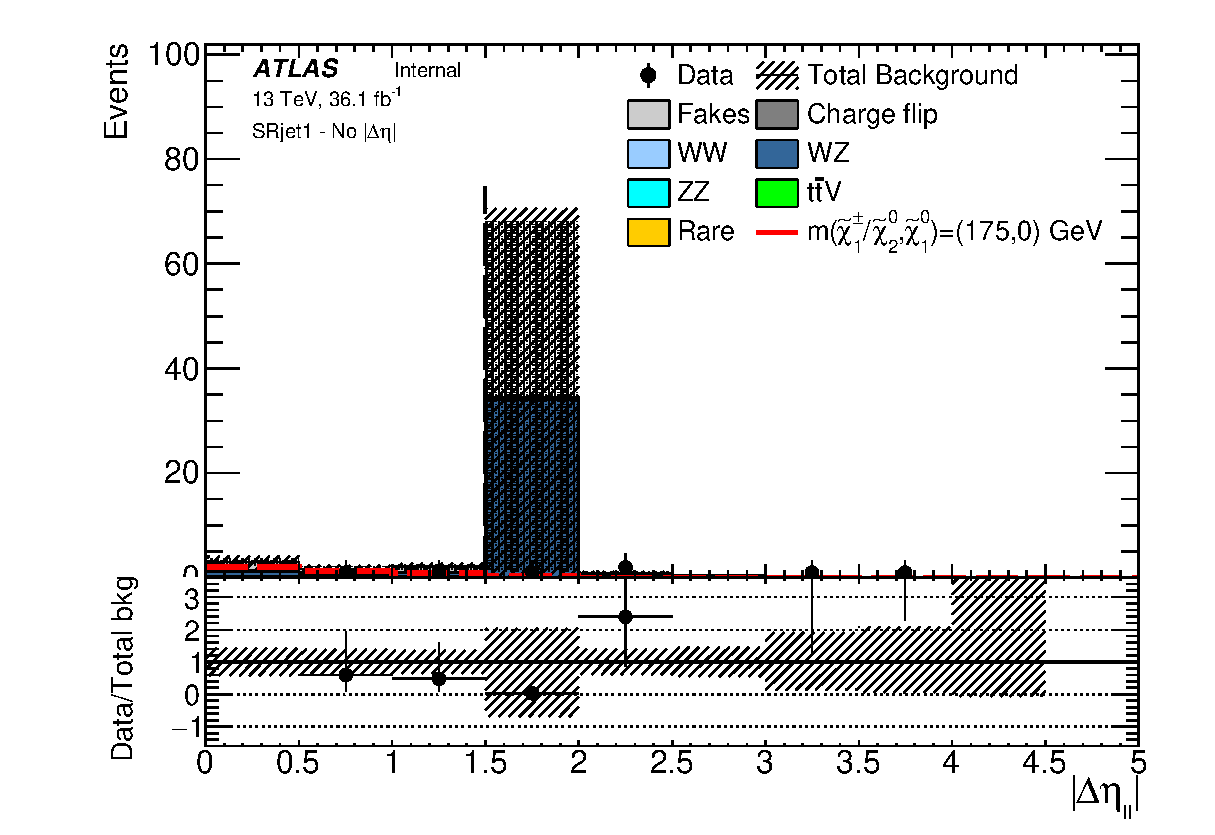
\includegraphics[width=0.45\textwidth]{data/plot/PlotsN1/all_DEtall_SRjet1_NoDEtall.eps}
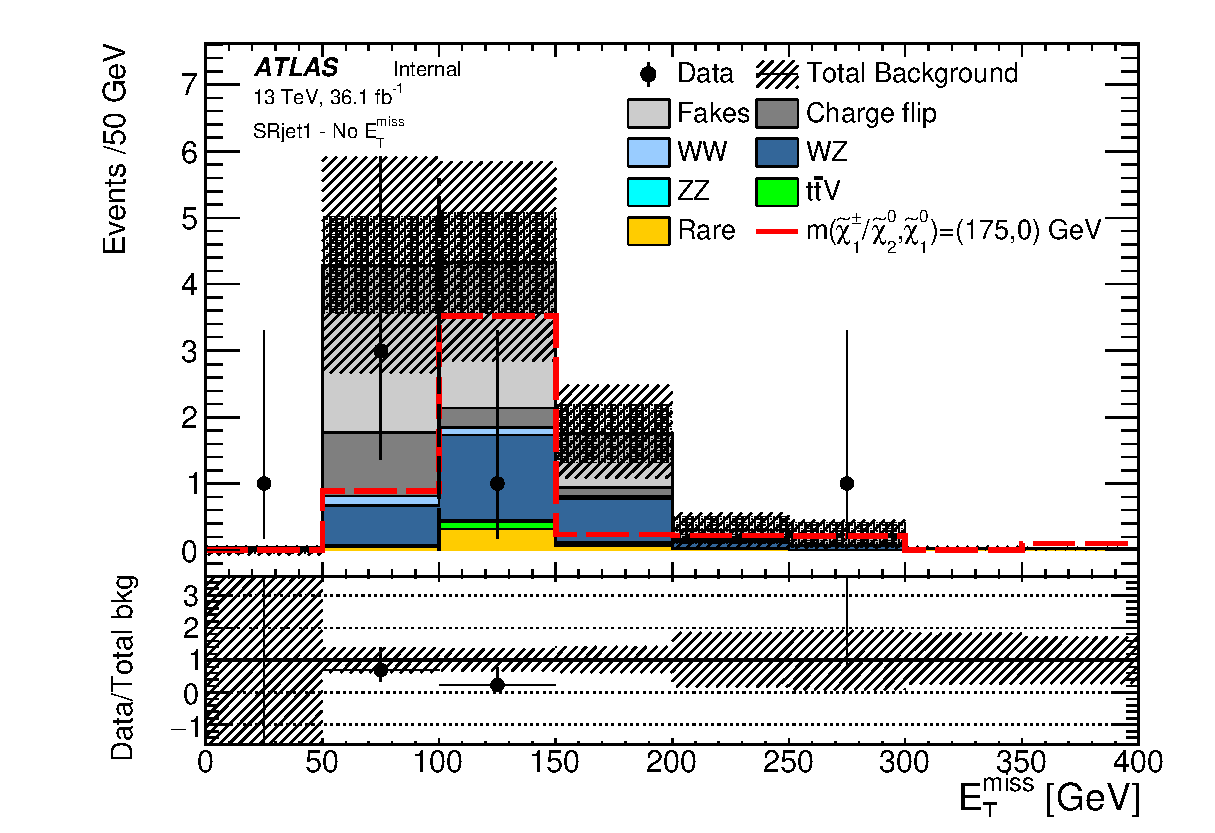
\includegraphics[width=0.45\textwidth]{data/plot/PlotsN1/all_Met_SRjet1_NoMet.eps} \\
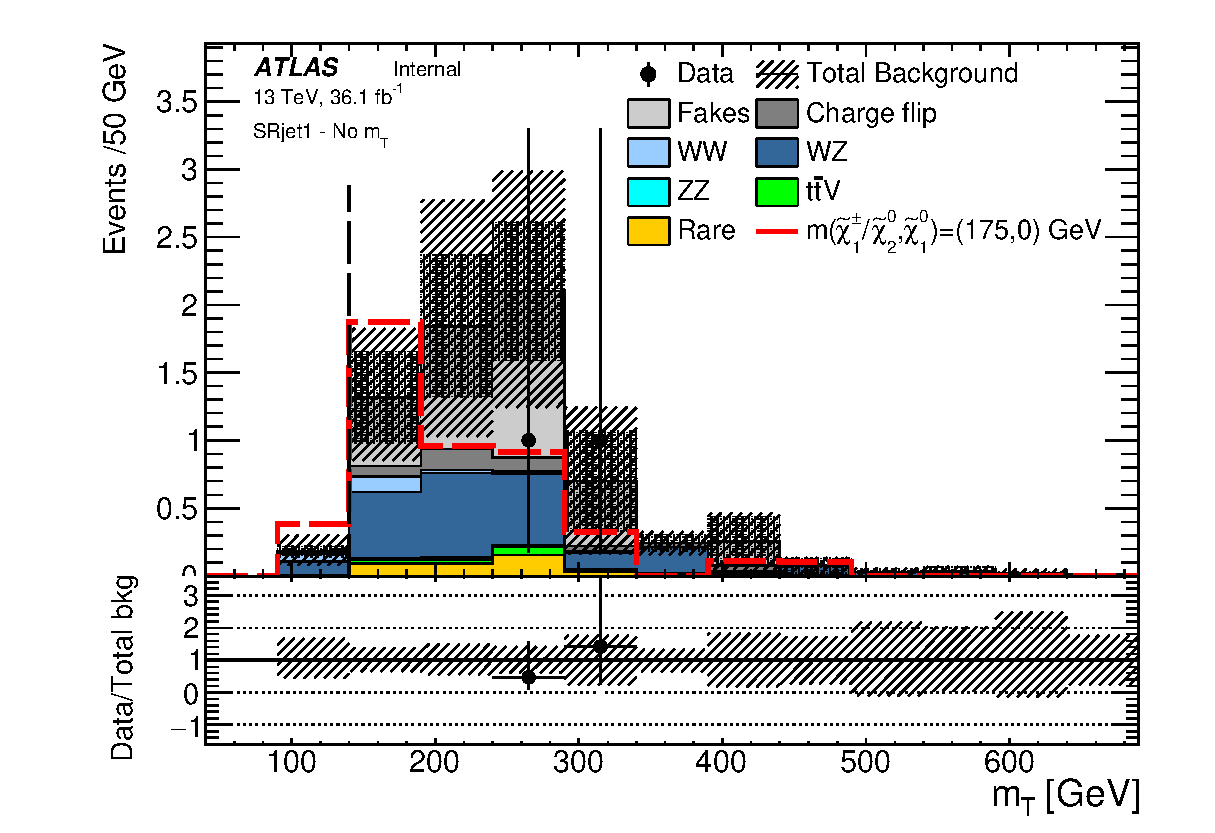
\includegraphics[width=0.45\textwidth]{data/plot/PlotsN1/all_Mt_SRjet1_NoMt.eps}
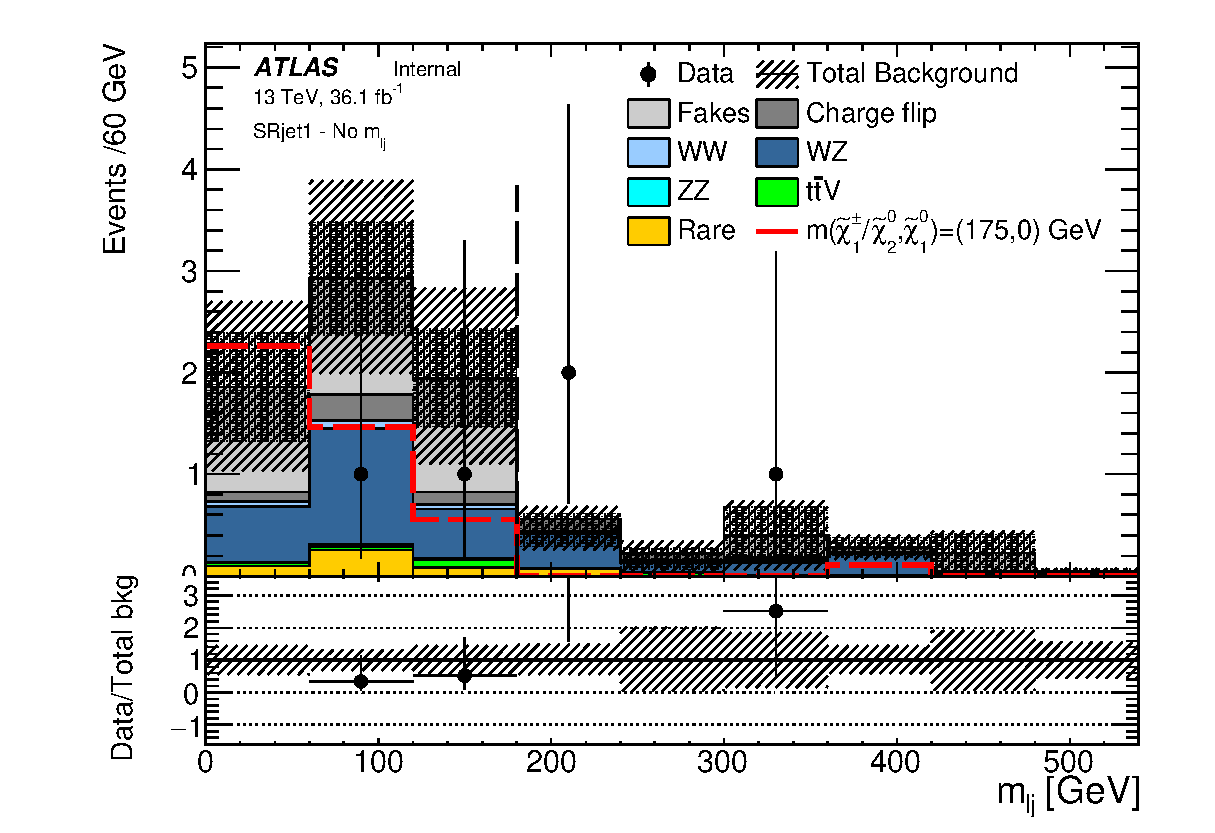
\includegraphics[width=0.45\textwidth]{data/plot/PlotsN1/all_Mlj_SRjet1_NoMlj.eps} \\
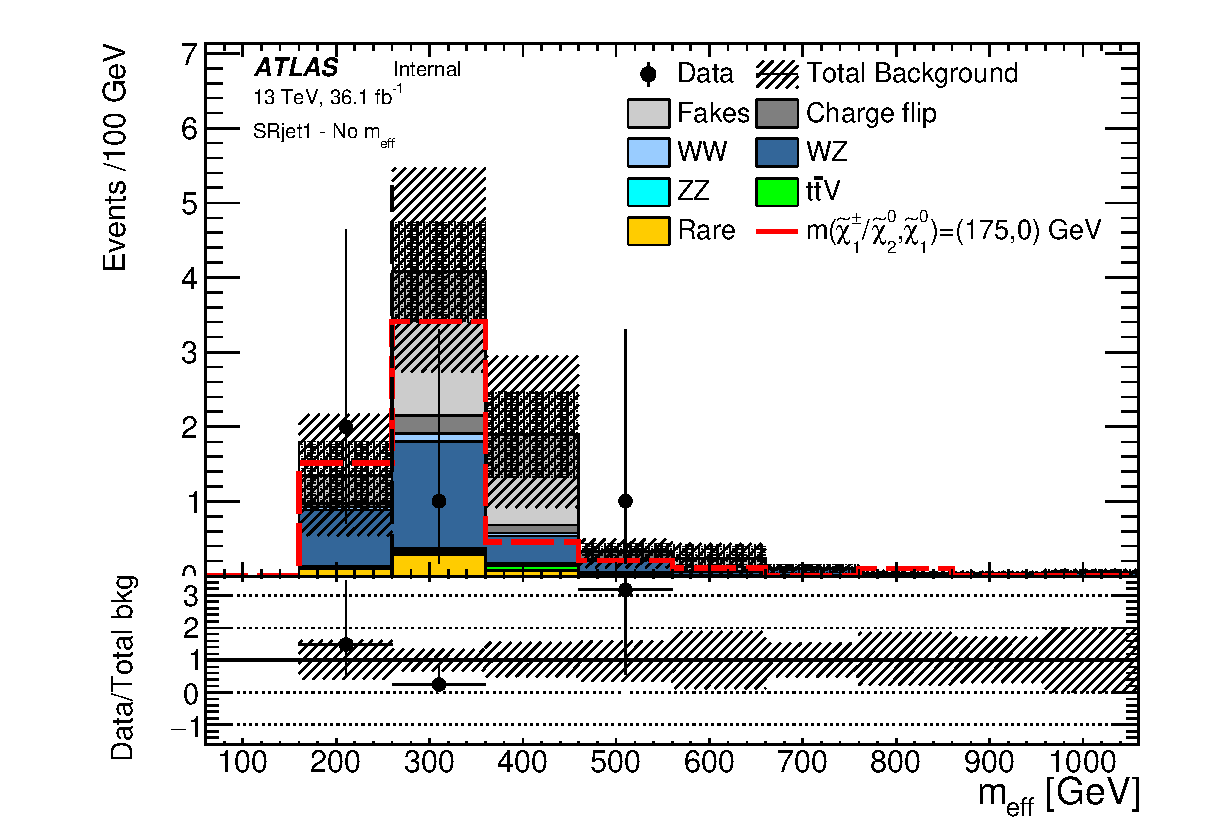
\includegraphics[width=0.45\textwidth]{data/plot/PlotsN1/all_Meff_SRjet1_NoMeff.eps}
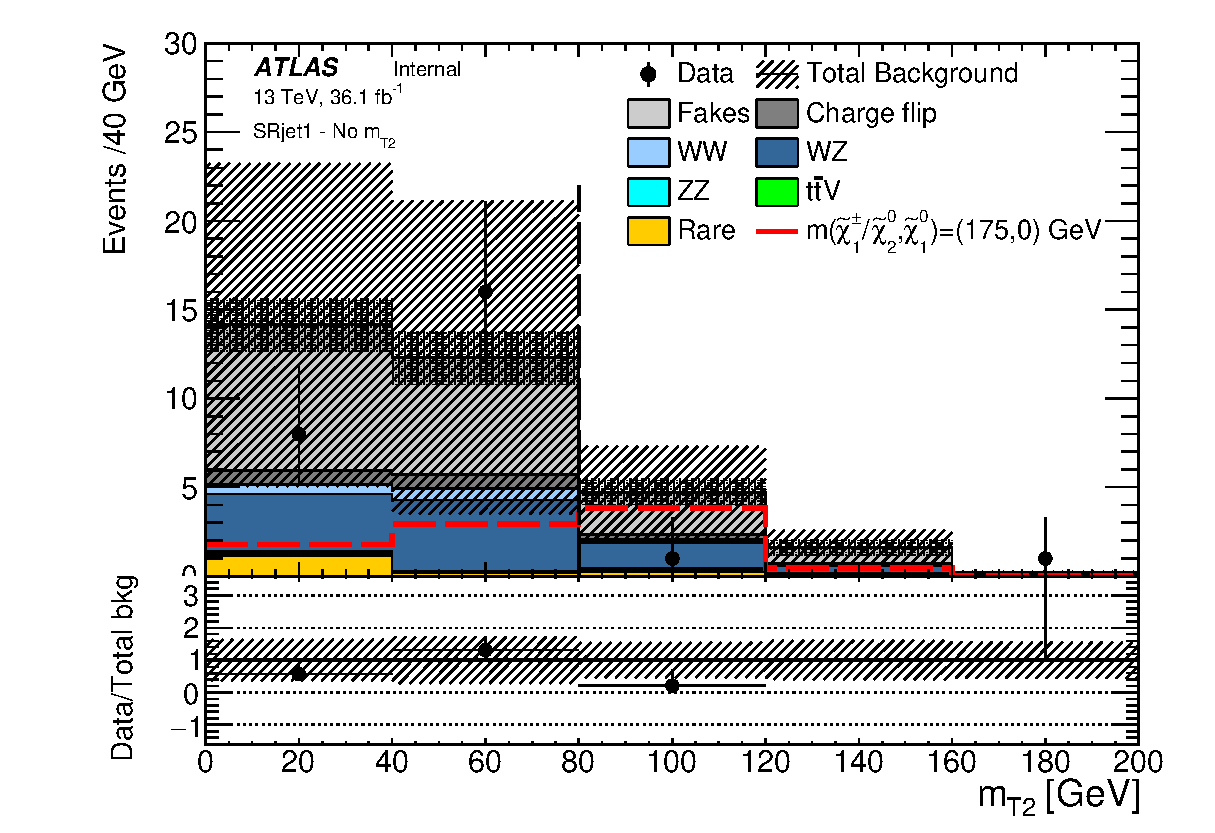
\includegraphics[width=0.45\textwidth]{data/plot/PlotsN1/all_Mt2_SRjet1_NoMt2.eps}
\caption{N-1 plots for different variable distributions in the SRjet1 for the background estimation and the data. The signal of the mass point with the highest significance ($m_{\tilde{\chi}_1^\pm , \tilde{\chi}_2^0}$,$m_{\tilde{\chi}_1^0}$) = (175,0) is shown by the red dashed line. The internal shaded area refers to the statistical uncertainties, while the external shaded area refers to the total uncertainty. The vertical dashed line shows the SR cut of that variable. The lower plot shows the ratio of data yields with respect to the total background predictions. The plots are made by Dr. Daniela Paredes \cite{Wh}.}
\label{fig:result_Nminus1_1}
\end{figure}

\begin{figure}[htbp]
\centering
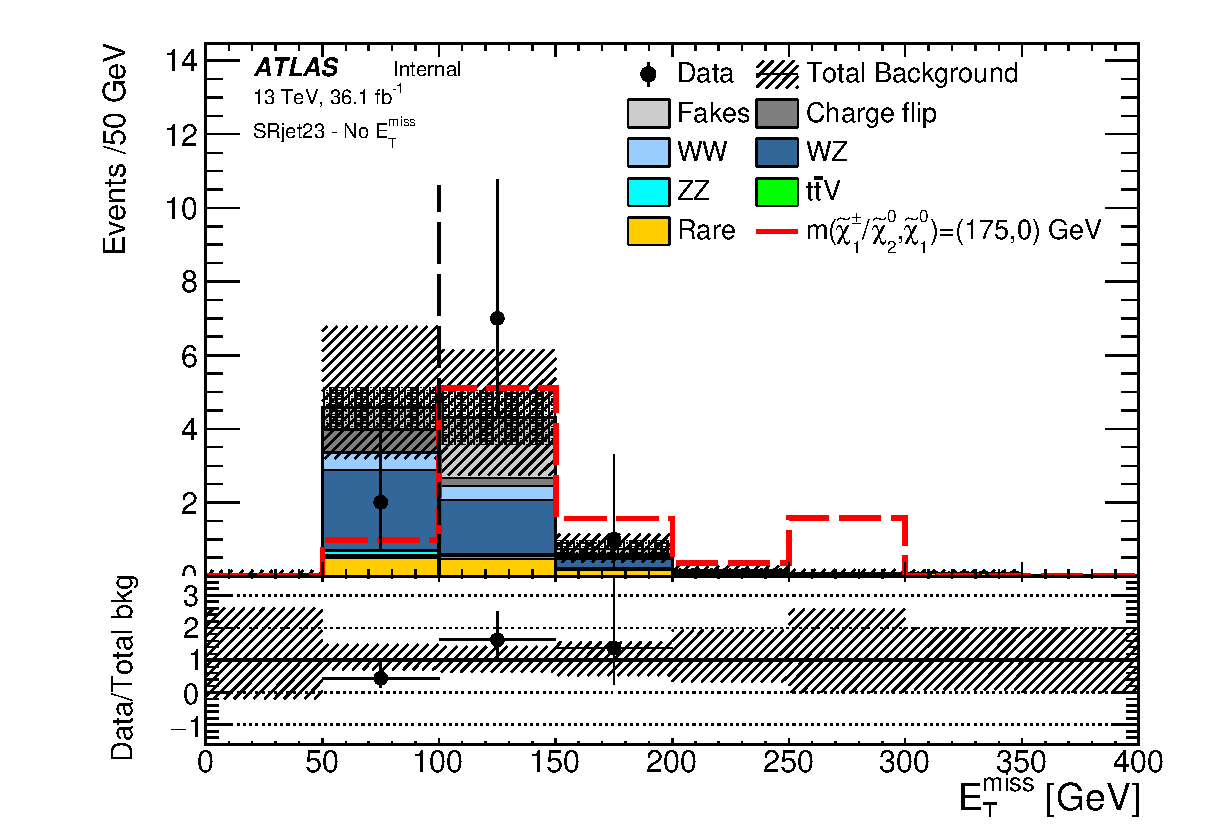
\includegraphics[width=0.45\textwidth]{data/plot/PlotsN1/all_Met_SRjet23_NoMet.eps}
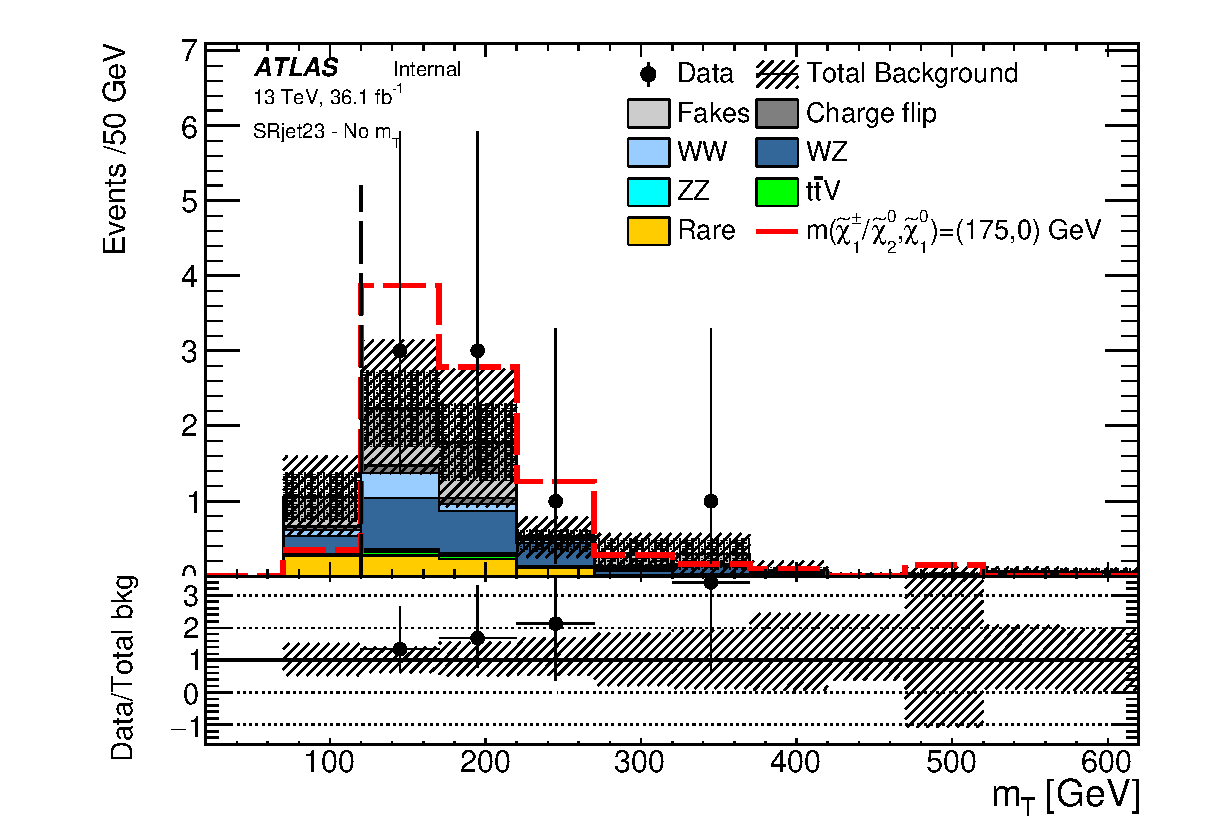
\includegraphics[width=0.45\textwidth]{data/plot/PlotsN1/all_Mt_SRjet23_NoMt.eps} \\
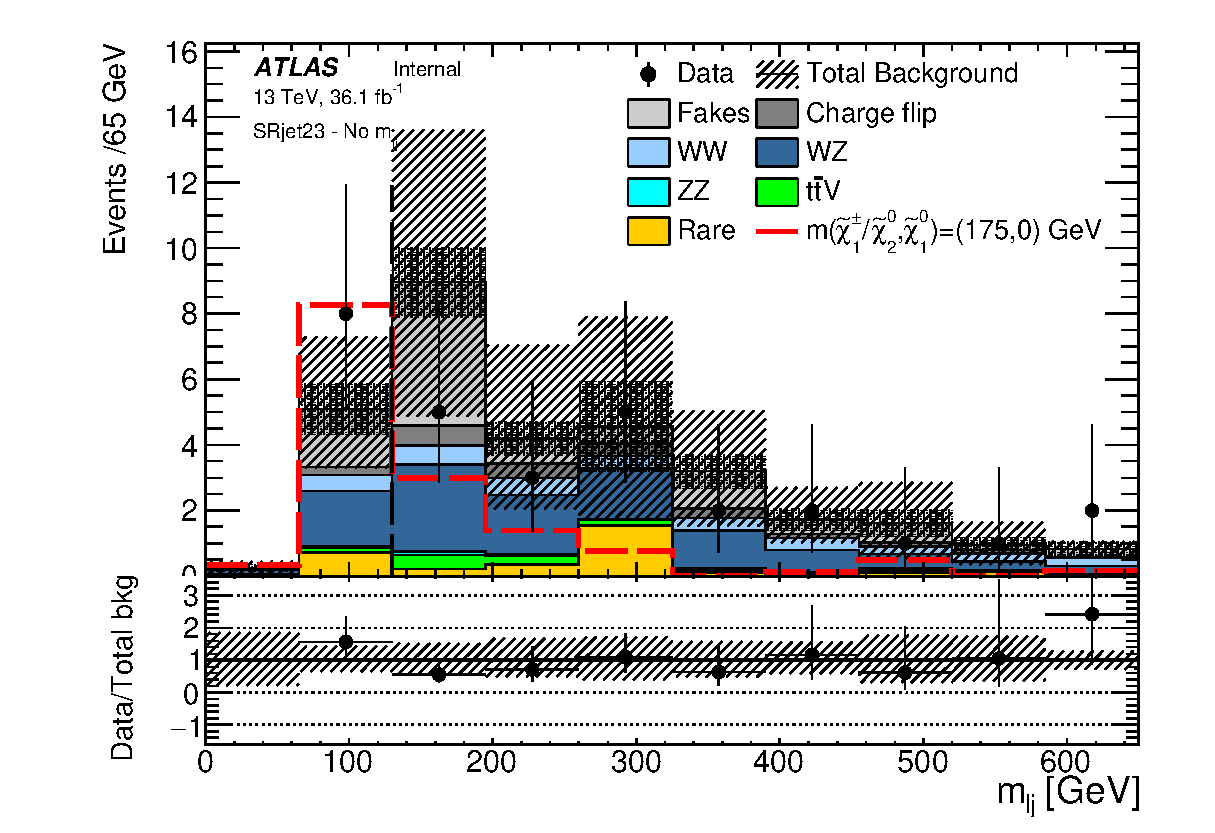
\includegraphics[width=0.45\textwidth]{data/plot/PlotsN1/all_Mlj_SRjet23_NoMlj.eps}
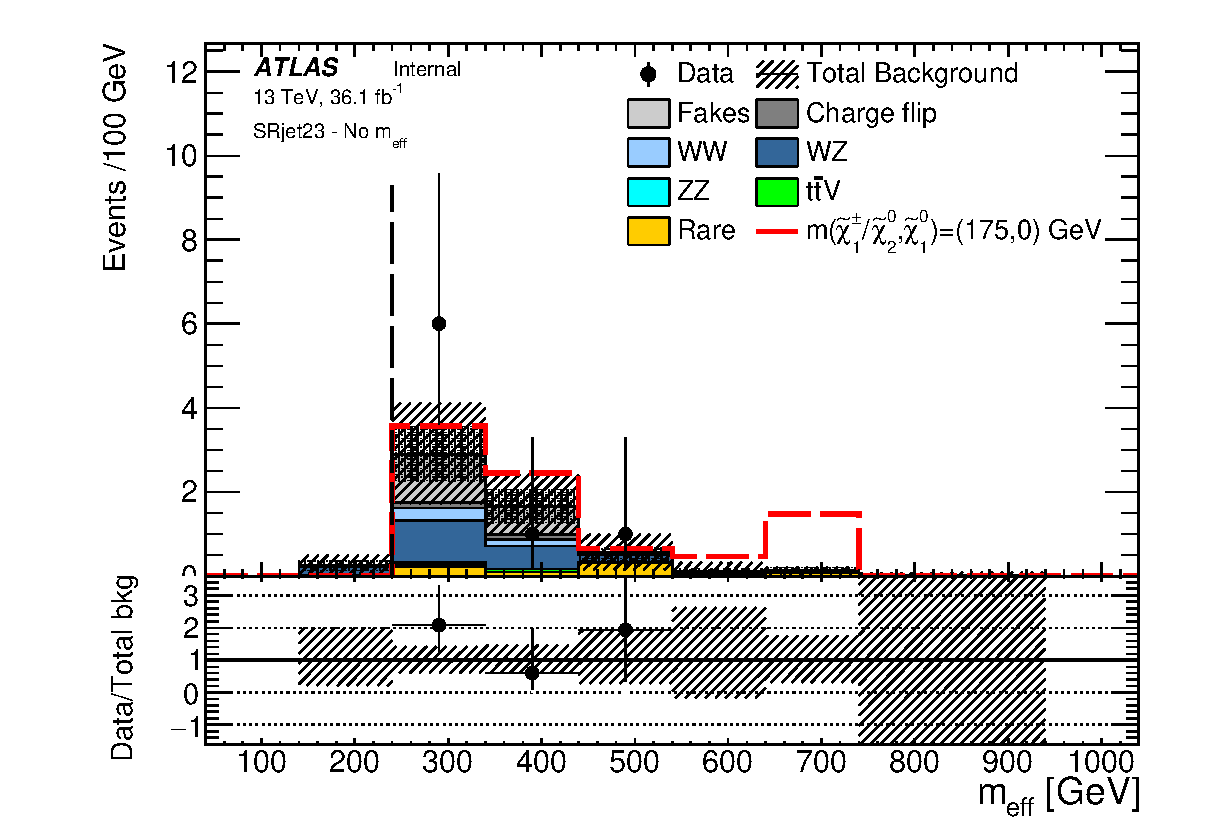
\includegraphics[width=0.45\textwidth]{data/plot/PlotsN1/all_Meff_SRjet23_NoMeff.eps} \\
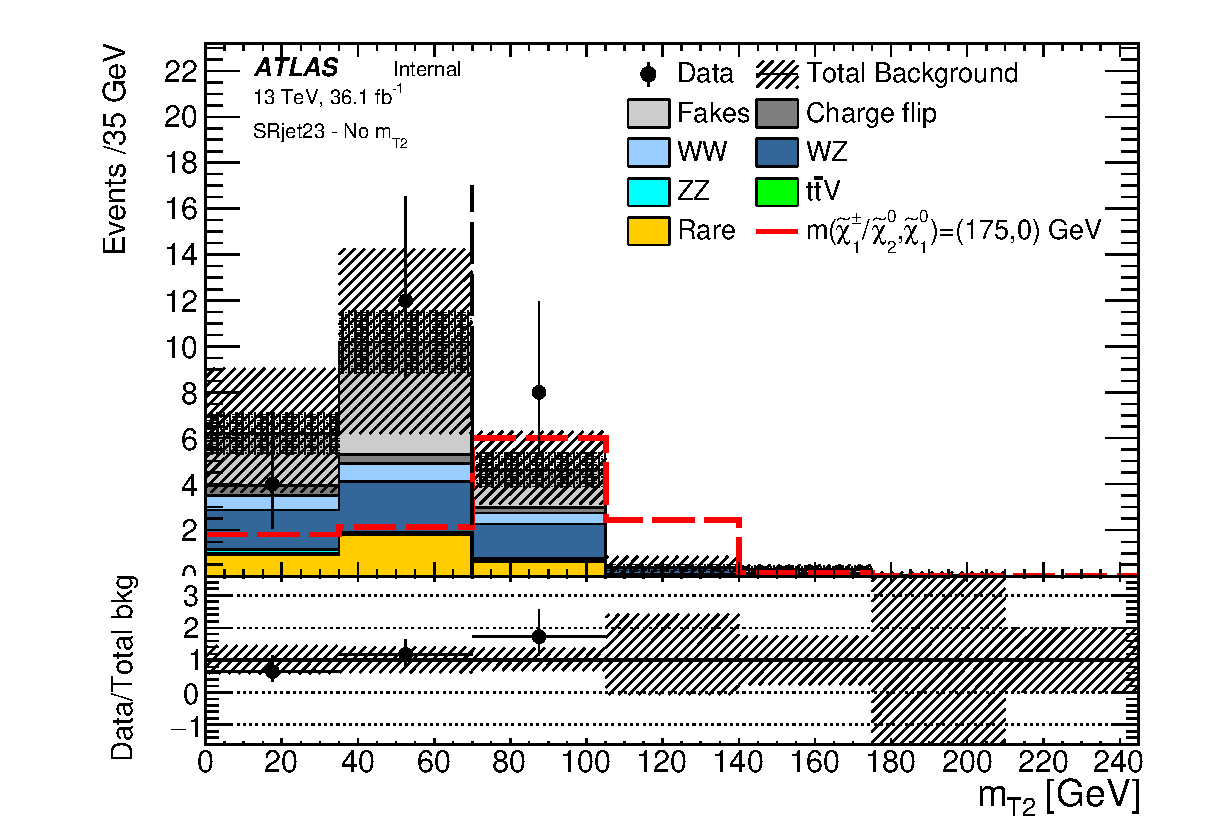
\includegraphics[width=0.45\textwidth]{data/plot/PlotsN1/all_Mt2_SRjet23_NoMt2.eps}
\caption{N-1 plots for different variable distributions in the SRjet23 for the background estimation and the data. The signal of the mass point with the highest significance ($m_{\tilde{\chi}_1^\pm , \tilde{\chi}_2^0}$,$m_{\tilde{\chi}_1^0}$) = (175,0) is shown by the red dashed line. The internal shaded area refers to the statistical uncertainties, while the external shaded area refers to the total uncertainty. The vertical dashed line shows the SR cut of that variable. The lower plot shows the ratio of data yields with respect to the total background predictions. The plots are made by Dr. Daniela Paredes \cite{Wh}.}
\label{fig:result_Nminus1_2}
\end{figure}

Table \ref{tab:result_upper_limit} shows the results of the model-independent fit.
The numbers in the first column are the upper limits on the observed visible cross-section $\sigma_{\text{vis}}$ at 95\% confidence level.
The second and third column show the upper limits on the observed ($S_{\rm obs}^{95}$) and expected ($S_{\rm exp}^{95}$) signal events respectively, at 95\% confidence level.
The fluctuations of the upper limits of $S_{\rm exp}^{95}$ are also shown, with $\pm 1\sigma$ excursions on the expectation of the background events.
The definition of the observed visible cross-section $\sigma_{\text{vis}}$ is the product of a BSM cross-section, the acceptance and the selection efficiency of a BSM signal.
The last column shows the discovery $p$-value ($p_0$).
It is the probability that the Standard Model background fluctuate to the observed number of events or higher.

\begin{table}[htbp]
\begin{center}
\begin{tabular}{|l|cccc|}
\hline
& $\langle \sigma_{\text{vis}} \rangle_{\rm obs}^{95}$[fb]  &  $S_{\rm obs}^{95}$  & $S_{\rm exp}^{95}$ & $p_0$ \\
\hline
\hline
SRjet1  & $0.12$ & $4.2$ & $ { 6.1 }^{ +2.7 }_{ -1.5 }$ & $ 0.50$ \\
\hline
SRjet23 & $0.27$ & $9.9$ & $ { 6.6 }^{ +3.4 }_{ -1.1 }$ & $ 0.17$ \\
\hline
\end{tabular}
\caption{
From left to right:
95\% confidence level upper limits on the visible cross section ($\langle \sigma_{\text{vis}} \rangle_{\rm obs}^{95}$)
and on the observed number of signal events ($S_{\rm obs}^{95}$).
The third column ($S_{\rm exp}^{95}$) shows the 95\% confidence level upper limit on the expected number of signal events,
with $\pm 1\sigma$ excursions on the expectation of the background events.
%The last two columns indicate the $CL_B$ value, i.e. the confidence level observed for the background-only hypothesis.
The last column shows the discovery $p$-value ($p_0$).}
\label{tab:result_upper_limit}
\end{center}
\end{table}

Figure \ref{fig:result_exclusion_limit} shows the expected and observed exclusion limits on the masses of $m_{\tilde{\chi}_1^\pm, \tilde{\chi}_2^0}$ and $m_{\tilde{\chi}_1^0}$ at the 95\% confidence level.
The mass points inside the curve are excluded.
The exclusion limits are calculated by combining the two signal regions.
Compared with other channels in Wh search \cite{Wh}, our same-sign channel is sensitive in the low $m_{\tilde{\chi}_1^\pm, \tilde{\chi}_2^0}$ region and the compressed region described in section \ref{sec:Wh_signal}.
The exclusion limits for the masses $m_{\tilde{\chi}_1^\pm, \tilde{\chi}_2^0}$ and $m_{\tilde{\chi}_1^0}$ supersede the run 1 results \cite{run1}.

\begin{figure}[htbp]
\centering
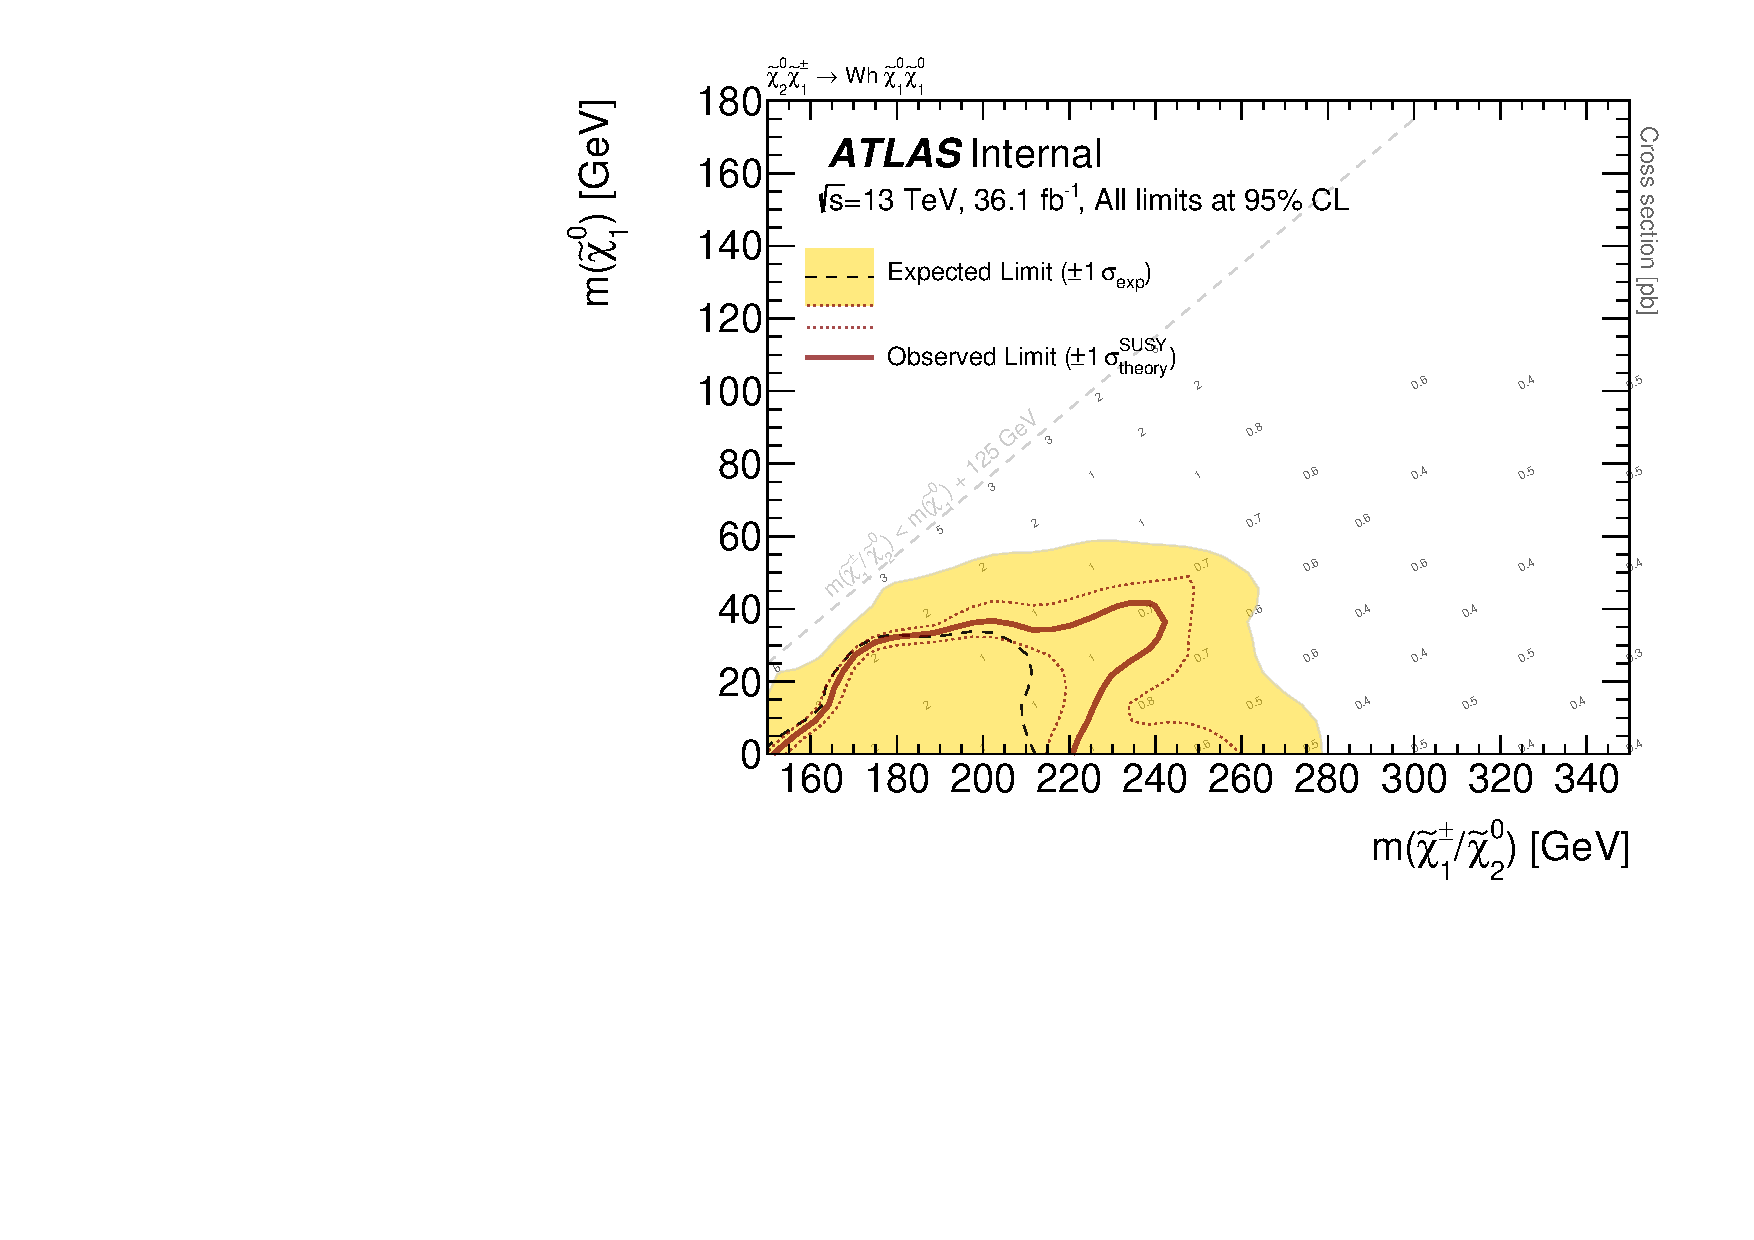
\includegraphics[width=\textwidth]{data/plot/HistFitterResults/contourPlotterWhSS_upperLimit.pdf}
\caption{The expected and observed exclusion limits for the combined SRjet1 and SRjet23 are shown. Experimental and theoretical systematic uncertainties are applied to background and signal samples and illustrated by the yellow band and the red dotted contour lines respectively. The red dotted lines indicate the $\pm 1 \sigma$ variation on the observed exclusion limit due to theoretical uncertainties on the signal cross-section. The upper limits for signal cross section at different mass points are also shown in grey numbers.}
\label{fig:result_exclusion_limit}
\end{figure}

%

\begin{table}
\begin{center}
\setlength{\tabcolsep}{0.0pc}
{\small
%%
\begin{tabular*}{\textwidth}{@{\extracolsep{\fill}}lrr}
\noalign{\smallskip}\hline\noalign{\smallskip}
{\bf table.results.yields channel}           & SRjet1            & SRjet23              \\[-0.05cm]
\noalign{\smallskip}\hline\noalign{\smallskip}
%%
Observed events          & $2$              & $8$                    \\
\noalign{\smallskip}\hline\noalign{\smallskip}
%%
Fitted bkg events         & $4.36 \pm 1.58$          & $5.92 \pm 1.27$              \\
\noalign{\smallskip}\hline\noalign{\smallskip}
%%
        Fitted Fakes events         & $1.07_{-1.07}^{+1.54}$          & $2.25 \pm 1.21$              \\
%%
        Fitted WZ events         & $2.07 \pm 0.44$          & $1.95 \pm 0.58$              \\
%%
        Fitted Rare events         & $0.43 \pm 0.13$          & $0.72 \pm 0.18$              \\
%%
        Fitted ttV events         & $0.11 \pm 0.05$          & $0.14 \pm 0.05$              \\
%%
        Fitted WW events         & $0.16 \pm 0.03$          & $0.52 \pm 0.07$              \\
%%
        Fitted ZZ events         & $0.05 \pm 0.03$          & $0.07 \pm 0.04$              \\
%%
        Fitted ChargeFlip events         & $0.47 \pm 0.07$          & $0.27 \pm 0.03$              \\
%%     
 \noalign{\smallskip}\hline\noalign{\smallskip}
%%
MC exp. SM events              & $6.74 \pm 2.18$          & $5.33 \pm 1.61$              \\
\noalign{\smallskip}\hline\noalign{\smallskip}
%%
        MC exp. Fakes events         & $3.30 \pm 2.10$          & $1.76 \pm 1.47$              \\
%%
        MC exp. WZ events         & $2.18 \pm 0.46$          & $1.85 \pm 0.57$              \\
%%
        MC exp. Rare events         & $0.44 \pm 0.13$          & $0.73 \pm 0.17$              \\
%%
        MC exp. ttV events         & $0.12 \pm 0.05$          & $0.14 \pm 0.05$              \\
%%
        MC exp. WW events         & $0.17 \pm 0.03$          & $0.51 \pm 0.07$              \\
%%
        MC exp. ZZ events         & $0.06 \pm 0.03$          & $0.07 \pm 0.04$              \\
%%
        MC exp. ChargeFlip events         & $0.47 \pm 0.07$          & $0.27 \pm 0.03$              \\
%%     \\
\noalign{\smallskip}\hline\noalign{\smallskip}
\end{tabular*}
%%%
}
\end{center}
\caption{Signal region: . Fit results for the electron (top part) and muon (bottom part) channels, for an integrated luminosity of $1035$.
The results are obtained from the control regions using the discovery fit (see text for details). The fit results of the loose-not-tight regions are not shown.
Nominal MC expectations (normalised to MC cross-sections) are given for comparison. 
The Monte Carlo QCD estimates are provided for illustrational purposes only, and are not used in the fit.
The errors shown are the statistical plus systematic uncertainties, except for the error on the background estimate in the signal region, which is the systematic uncertainty only.
Uncertainties on the fitted yields are symmetric by construction, 
where the negative error is truncated when reaching to zero event yield.
}
\label{table.results.systematics.in.logL.fit.table.results.yields}
\end{table}
%


%************************************************
\chapter{Conclusion}
\label{ch:conclusion}
%************************************************

Results of a search for the electroweak pair production of chargino and neutralino
($p + p \rightarrow \tilde{\chi}_1^\pm + \tilde{\chi}_2^0$) are presented in the Wh channel $\tilde{\chi}_1^\pm \rightarrow \tilde{\chi}_1^0 + W$ and $\tilde{\chi}_2^0 \rightarrow \tilde{\chi}_1^0 + h$ with same-sign leptons in the final states.
The dominant background is the fake lepton background, and the dominant irreducible background is the diboson processes, especially the WZ processes.
Two signal regions are defined and optimized for the compressed region where the mass difference between $\tilde{\chi}_1^\pm$/$\tilde{\chi}_2^0$ and $\tilde{\chi}_1^0$ is close to the Higgs mass 125 GeV.
No significant deviations from the SM predictions are observed, therefore new exclusion limits for the masses $m_{\tilde{\chi}_1^\pm, \tilde{\chi}_2^0}$ and $m_{\tilde{\chi}_1^0}$ are set, which supersedes the run 1 results \cite{run1}.
